\documentclass[a4paper,11pt]{article}
\usepackage[left=2.5cm, right=2.5cm, top=1.5cm, bottom=1.5cm]{geometry}
\usepackage{graphicx}
\usepackage{amssymb}
\usepackage{amsmath}
\usepackage{xcolor}
\usepackage{hyperref}
\usepackage{pythonhighlight}

\hypersetup{ %color attributes of citation, link, etc.
colorlinks=true,
linkcolor=blue,
filecolor=gray,
urlcolor=blue,
citecolor=blue,
}

\setlength{\parindent}{0pt}

% \usepackage[active,tightpage]{preview}
% \renewcommand{\PreviewBorder}{1in}
% \newcommand{\Newpage}{\end{preview}\begin{preview}}

\newcommand{\matlab}{\textsc{Matlab}} %very important and totally necessary addition
\newcommand{\parallelsum}{\mathbin{\!/\mkern-5mu/\!}}

\newcommand\Item[1][]{%
  \ifx\relax#1\relax  \item \else \item[#1] \fi
  \abovedisplayskip=0pt\abovedisplayshortskip=0pt~\vspace*{-\baselineskip}}

%'codify' text for snippets
\usepackage{xcolor}
\definecolor{codegray}{gray}{1}
\newcommand{\code}[1]{\colorbox{codegray}{\texttt{#1}}}


\graphicspath{ {../images/} }
           
\begin{document}
\title{\LARGE{\textbf{Monophonic Mechatronic Chordophone}}}
\author{Niels Clayton : 300437590\\\textbf{Group Members:} Daniel Eisen \& Nickolai Wolfe}

\date{}
\maketitle
\hrule

\section{Introduction}

The field of mechatronic instruments aims to expand upon the human experiences of composing and performing music. Mechatronic instruments have the ability assist and enhance music playing, as well as producing new types of music that a human would find difficult or not be capable of replicating. \\

This report details the design of new picking and damping mechanisms for use within mechatronic chordophones. The motivations for theses designs will be based upon a previously completed review of the literature with this field, and looks to expand upon and improve existing designs.

\section{Design Motivations}\label{S:motivations}

The designs developed within this report have been specified to meet the following requirements:

\begin{itemize}
  \item Return string to it's static state within 0.25s of a pick operation 
  \item Achieve 120 pick damp cycles per minute
  \item Achieve At least 3 definable picking volumes
\end{itemize}

Aside from the provided requirements, existing literature was reviewed along with in-person demonstrations of existing chordophones. This this design limitations were identified for further development within this report. These improvements will focus on the usability of the picking and damping hardware, and look to improve the acoustic qualities of these elements.

\subsection{Identified Picker Design Motivations}\label{S:motivations_pick}

Based on existing literature, picking mechanisms such as the "pick-wheel" \cite{Carnegie2017} have been identified to be the most robust and adaptable picking mechanism. These mechanisms are designed around a rotating drum that has a selection of picks evenly spaced around it's exterior. Due to the construction of this picking mechanism, it lends itself to very simple and easy to control actuation, at relatively high speeds. \\

The "pick-wheel" mechanism is not without it's faults however. Due to the inclusion of multiple picks per rotation, any misalignment of a pick with respect to the others will lead to a substantial and audible difference in the picking tone (often referred to as a "galloping" sound). In tandem with this issue of pick alignment it was also identified that current "pick-wheel" designs suffered from the picks displacing over time, requiring continual re-adjustment to maintain performance.

It was also personally observed that during the picking operation of the MechBass \cite{McVay2015}, a loud audible clicking sound could be heard from each of it's pick wheels. This was identified to be a result of the retuning motion of each pick striking the central plastic drum of the pick wheel.\\

Finally is was also identified that existing picker volume switching methods lacked robustness, and often placed the responsible actuator under continuous strain to maintain a position. An example of this is found within the MechBass \cite{McVay2015}, in which a servo is used to displace the height of the picker by rotating it's 'horn' to lever it upwards. This design of adjustment often seemed to be an afterthought to the design of the picker, and also did not pose great accuracy in regard to volume selection.


\subsection{Identified Damper Design Motivations}\label{S:motivations_damp}

It was identified from the existing literature that the operation of the damping mechanism has had very little exploration and development within the field. The majority of existing damping mechanisms focus on contacting the string at a single point with a damping medium to extract the energy from the string. In designs shown by Carnegie et al. \cite{Carnegie2017}, servo motors have been used to rotate this damping medium to contact the string. In the literature it was discussed that these single contact methods produce noticeable distortion over the pick-up due to displacement of the string upon contact. This has been found to result result in a 'popping' sound that can be visually identified within audio-visualisation software.\\

Meanwhile in designs produced by Trimpin \cite{kapur_history_nodate}, a dual acting 'pinching' solenoid solution was explored. This solution proposed the ability to provide a fast acting damping force to the string, without applying the previously discussed displacement to the string. This design however required the damping solenoids to be matched and aligned for ideal operation, and in it's current state produces a large amount of audible in person noise as the solenoids make contact. 

Our attempted designs will iterate upon this dual acting solenoid solution, looking to mitigate the issues of solenoid matching and collisions.


\section{Proposed System Designs}

This section will display and discuss the designs that have been developed, and the solutions they pose in regards to the aforementioned issues discussed in Section \ref{S:motivations}.

\subsection{Proposed Picker Design}

As discussed in Section \ref{S:motivations_pick}, the identified issues with the existing "pick-wheel" design are as follows:

\begin{itemize}
  \item Misalignment of the picks
  \item Displacement of the picks over time
  \item Audible "clicking" sound due to pick rebound with "pick-wheel"
  \item Increased volume adjustment robustness
\end{itemize}

To address the misalignment of the picks and mitigate the "galloping" sound produced by existing pick designs, the pick-wheel barrel is design to be 3D printed with a slot that matches the dimensions of the picks. This slot will allow for precise and repeatable placement of the picks around the wheel, and will prevent rotation of the picks during usage. This can be clearly seen in Figure \ref{F:pic_assembly}, annotated as the key slot.\\

In order to mitigate the displacement of the picks over time, the pick clamping mechanism was adapted to extend over a greater portion of the pick body. This is designed to make greater contact with the pick, and make it less likely to be displaced by a picking action. This can be clearly seen in Figure \ref{F:pic_assembly}, annotated as the clamp.\\

Finally the audible clicking sound produced by picking backlash was mitigated through the introduction of a cushioning/damping medium. This damping medium will be placed between the pick and the 3D printed barrel to suppress the this audible click. Another cushion will also be placed at the interface between the pick and the clamp. This cushion will will damp any other backlash generated, and will also have the affect of increasing the area of contact between the clamp and the pick, thereby decreasing the likelihood of displacement. This can be clearly seen in Figure \ref{F:pic_assembly}, annotated as the silicone cushions.\\

In regards to the volume adjustment, it was important that it would not present as an afterthought to the picking mechanism, and would allow for robust and precise adjustment of the picker volume. This was achieved through the use of a rack and pinion gearing mechanism attached to a servo motor. The use of a rack and pinion removes the continuous holding strain required for the servo to vertically displace the picker. With our design, once a volume level has been selected no force is required to maintain that volume level. Because of this gearing mechanism, this design will be repeatable and it can be guaranteed that a known rotation will provide a known displacement and volume change. It can also be noted that the use of a rack and pinion gives great control over the volume selection of the picker, which can also be varied through the selection and use of differing pinions if desired. An overview of this design can be seen in Figure \ref{F:vol_assembly}, in which the rotation to linear displacement relationship has been displayed. 

\begin{figure}[h!]
  \begin{center}
    \includegraphics[width=0.4\textwidth]{picker_assembly.png}
    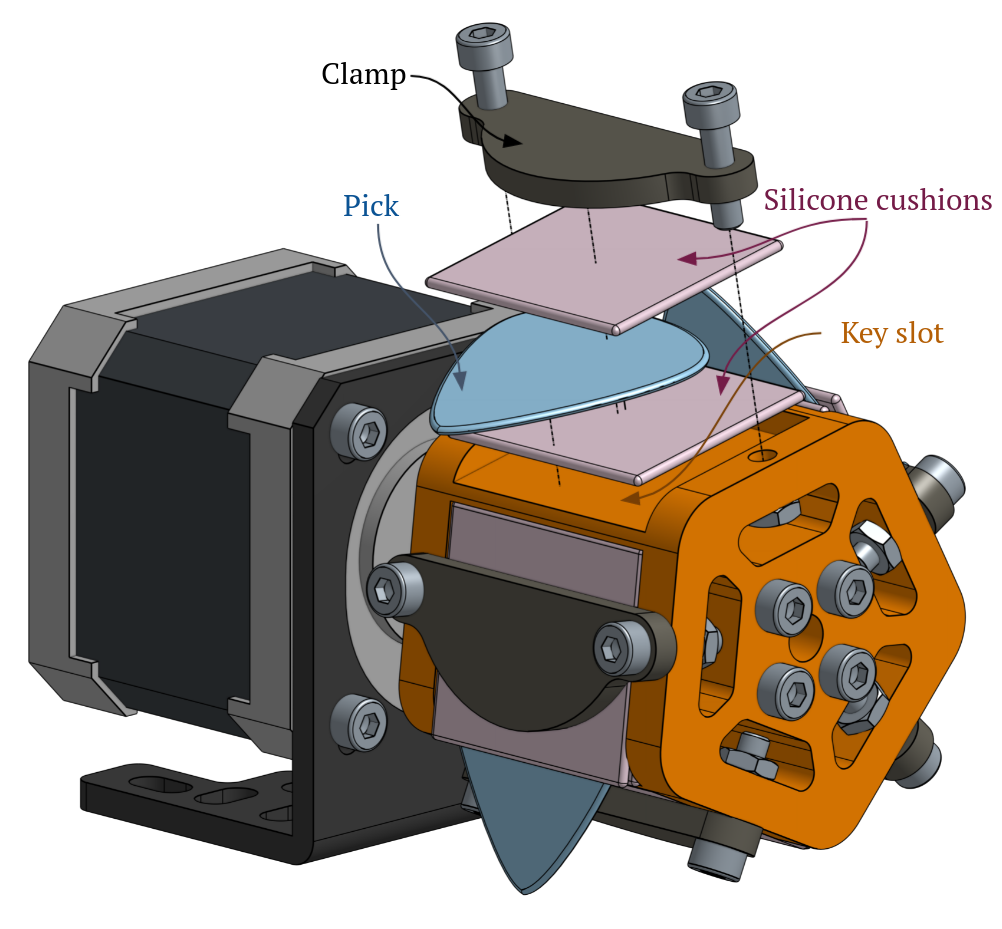
\includegraphics[width=0.4\textwidth]{picker_explode.png}
    \label{F:pic_assembly}
    \caption{Improved picker assembly design with exploded assembly view}
  \end{center}
\end{figure}

\begin{figure}[h!]
  \begin{center}
    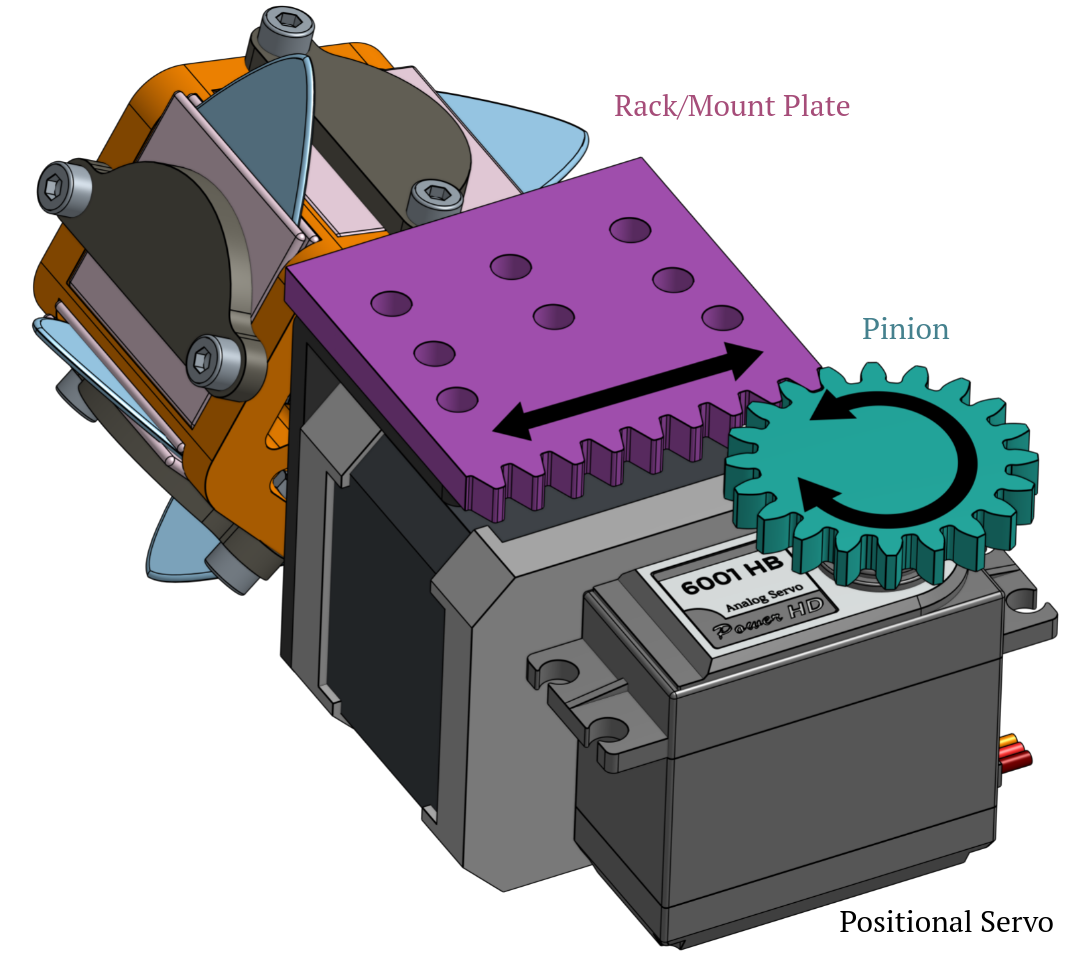
\includegraphics[width=0.4\textwidth]{volume_explode.png}
    \label{F:vol_assembly}
    \caption{Improved volume adjustment design}
  \end{center}
\end{figure}


\subsection{Proposed Damper Design}'

As discussed in Section \ref{S:motivations_damp}, the identified issues with the existing damper design are as follows:

\begin{itemize}
  \item Damping solenoids must be matched and aligned
  \item Audible sound generated when opposing solenoids collide
\end{itemize}

To address the issues outlined above, the damping interface was mounted on a 3D printable leaf spring. By mounting said leaf spring on the heads of the two opposing dampers, a damping operation will compress the two springs together on the string. Due to the spring interface the matching and alignment of the damping solenoids becomes less crucial, as any difference in the force applied, or the location of that force will be equalised through the spring. This will allow for damping of the picked string, without causing a displacement of the string.

The design of the spring contact is also such that it will have a large contact surface with the string. This will prevent the damper from actuating at the node of an oscillation, causing it to ineffective.\\

Finally the design of this damper is such that the damping interface material, and the leaf spring itself can be easily exchanged without the disassembly of the damping system, allowing for easy testing of a wide range of interface materials and spring designs. The implementation of this design, and an 'exploded' view detailing it's components can be seen in Figure \ref{F:damp_assembly}.

\begin{figure}[h!]
  \begin{center}
    \includegraphics[width=0.4\textwidth]{damper_assembly.png}
    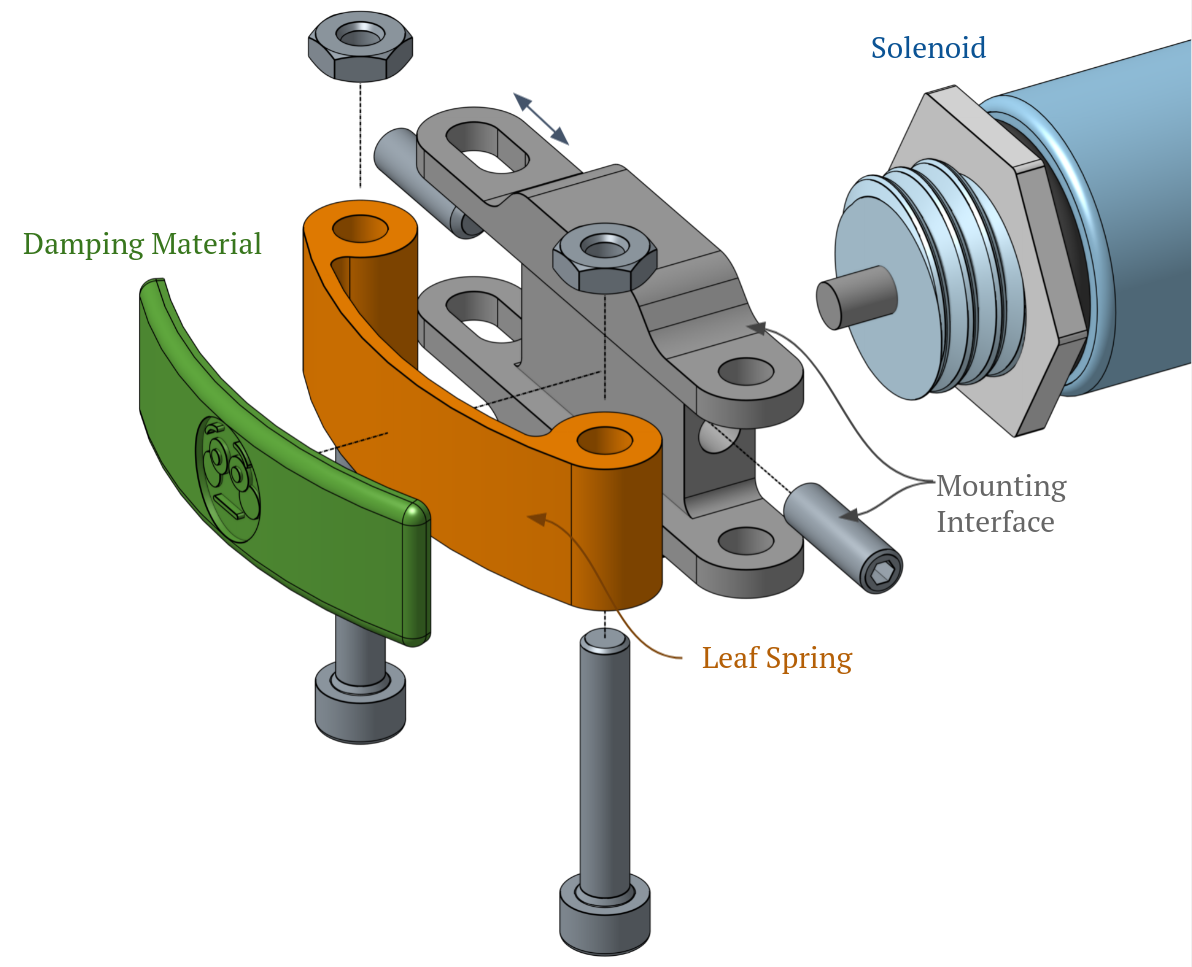
\includegraphics[width=0.4\textwidth]{damper_explode.png}
    \caption{Improved damper assembly design with exploded assembly view}
  \end{center}
  \label{F:damp_assembly}
\end{figure}

\subsection{Overall System Implementation}

The complete system implementation can be seen depicted in Figure \ref{F:full_assembly}. In this figure, the picking and damping mechanisms can be seen mounted to an aluminium extrusion, along with an magnetic pick-up. It should be noted that the mounting of the picker and damper allow for their placement anywhere along the length of the extrusion, allowing for the magnetic pick-up to be placed as far away from sources of electromagnetic noise as possible.

\begin{figure}[h!]
  \begin{center}
    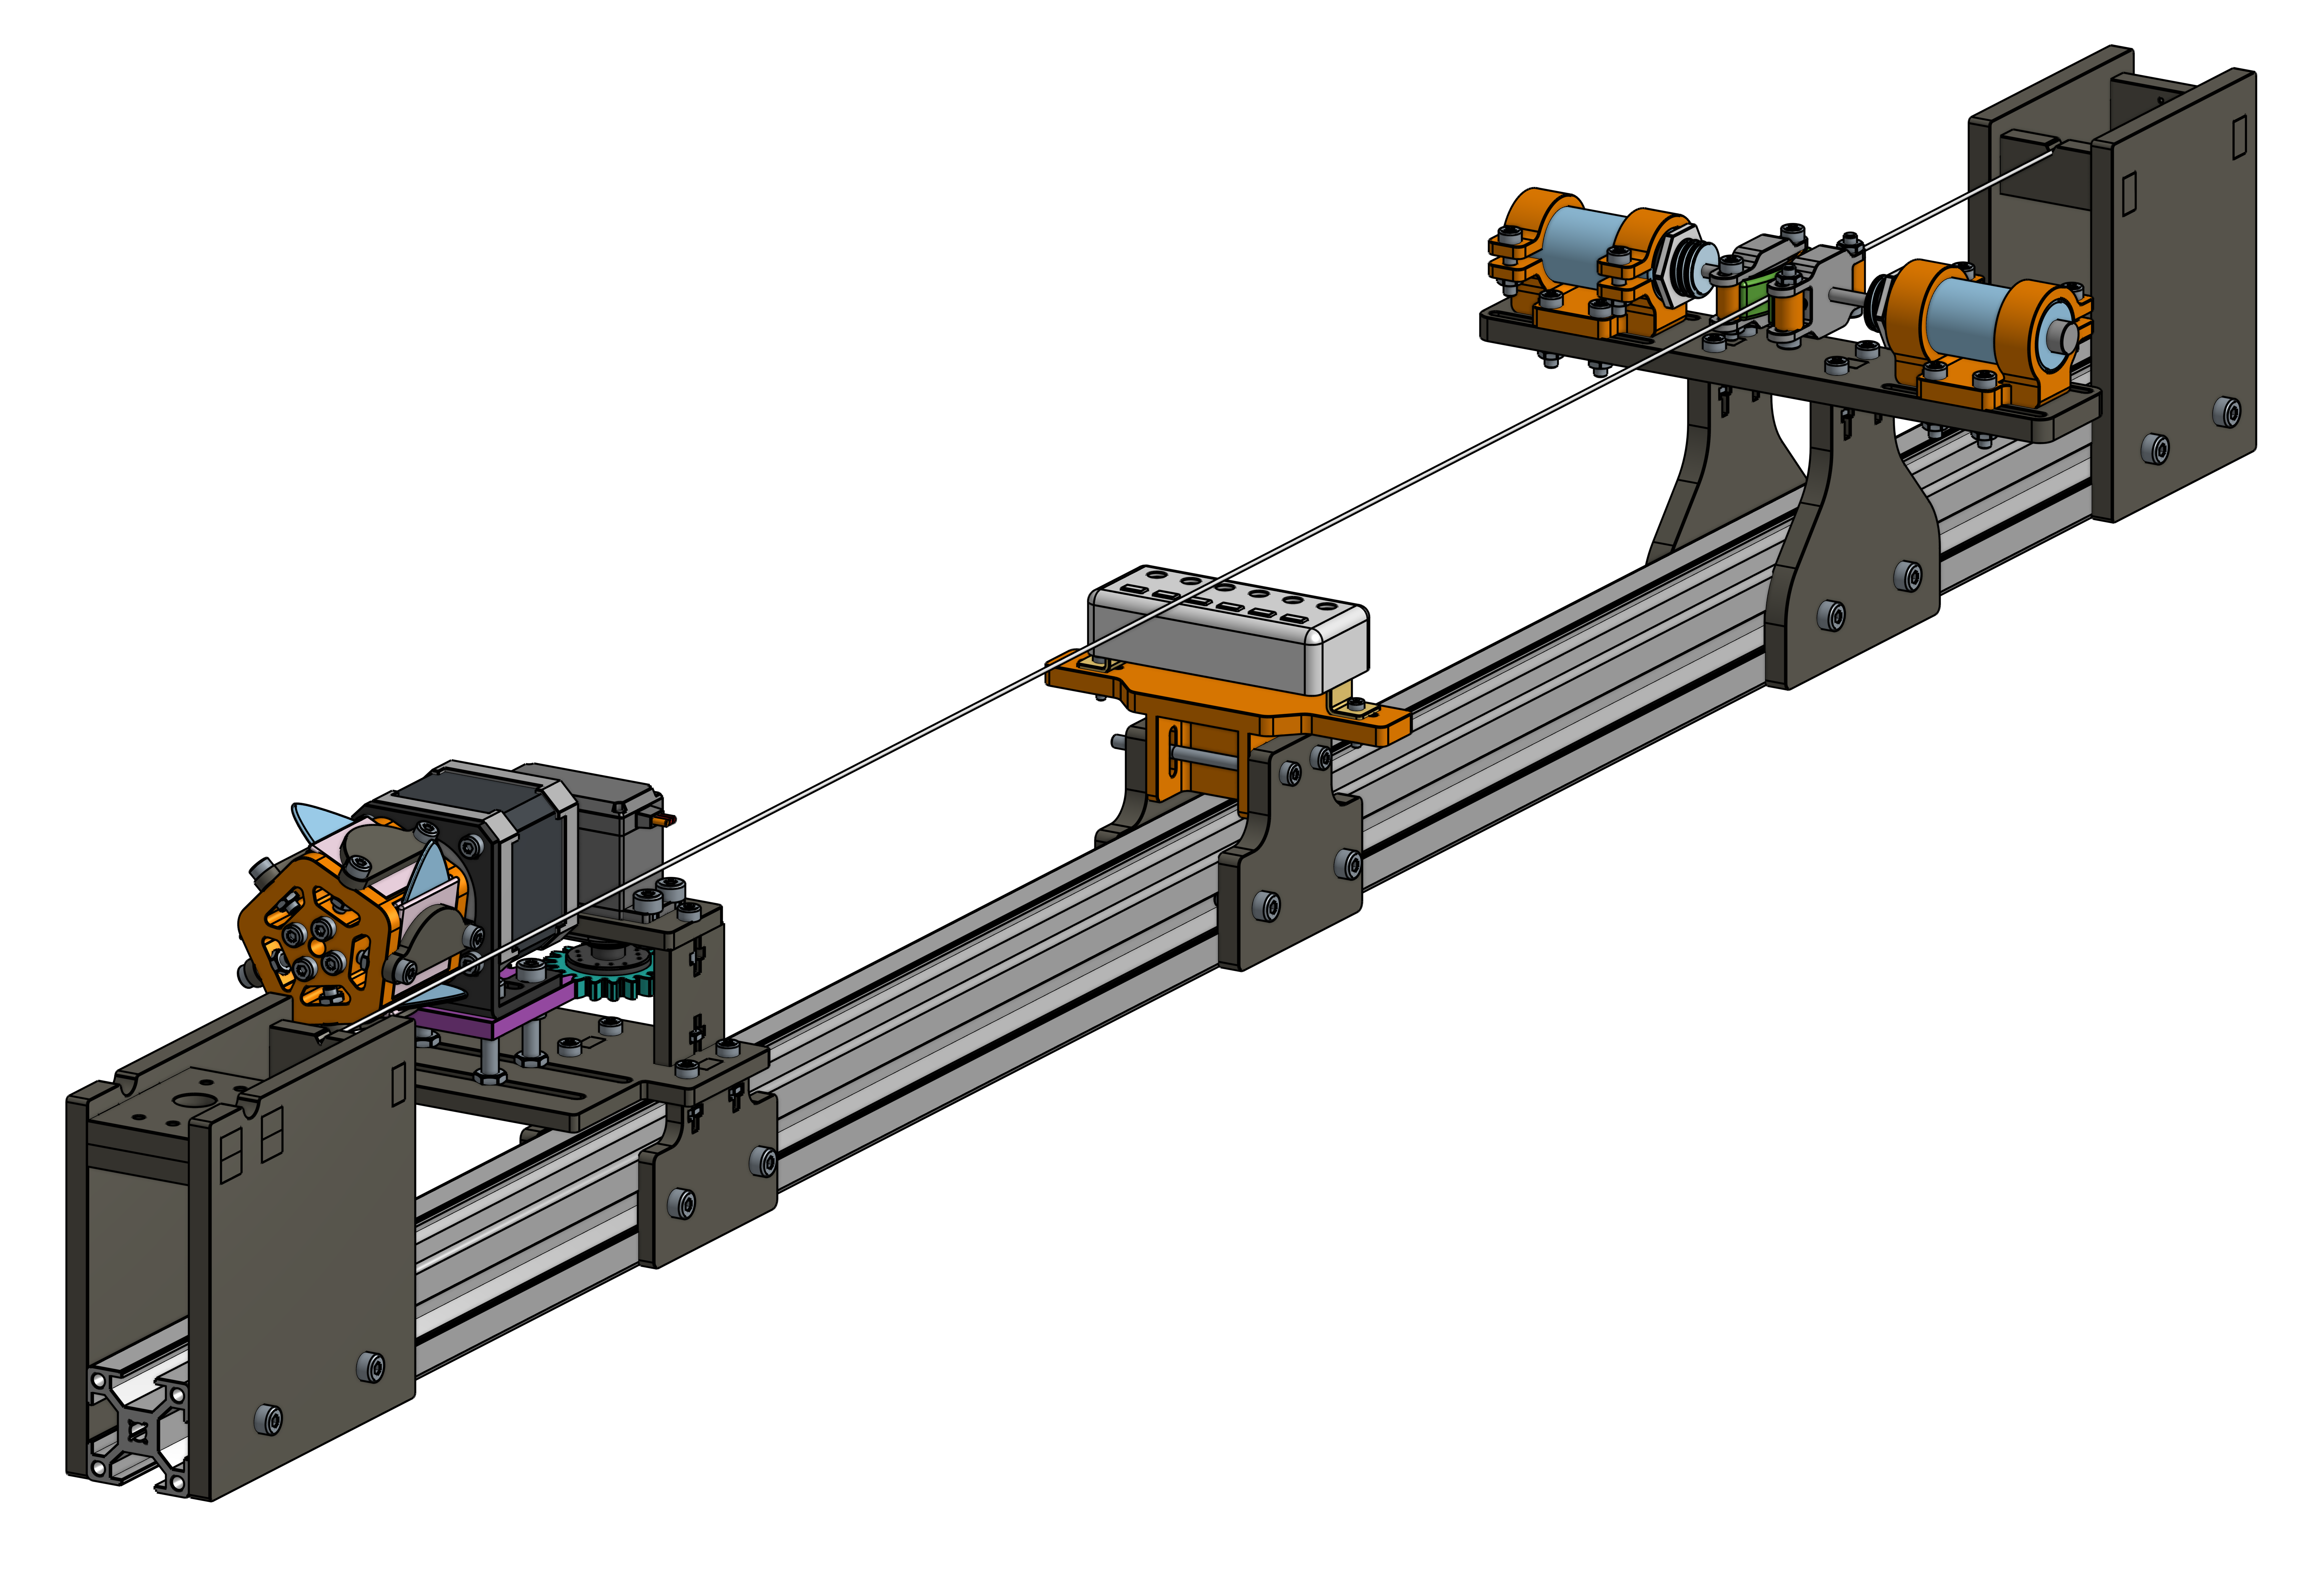
\includegraphics[width=0.7\textwidth]{picker_damper_full.png}
    \caption{Complete System Implementation}
  \end{center}
  \label{F:full_assembly}
  \vspace{-20pt}
\end{figure}


\subsection{Application Interface (API)}

To facilitate interaction with our designed picker and damper, as clean and easy to use application interface (API) has been developed. This API defines a header library each for the picker, the volume control, and the damper. These headers each implement an initialisation  function to set up the hardware, and an action function to perform a provided task. It should also be noted the the volume control library also provides a linearly spaced selection of 12 volumes that can be used. \\

As simple implementation of these headers is shown in Figure \ref{F:code}, in which all three libraries are used to implement a \code{play\_note} function. This function takes in a specified volume, sustain period, and damper active period, and will then select the provided volume, pick the note, and apply the damping after a given time.

\begin{figure}[h!]
  \begin{center}
    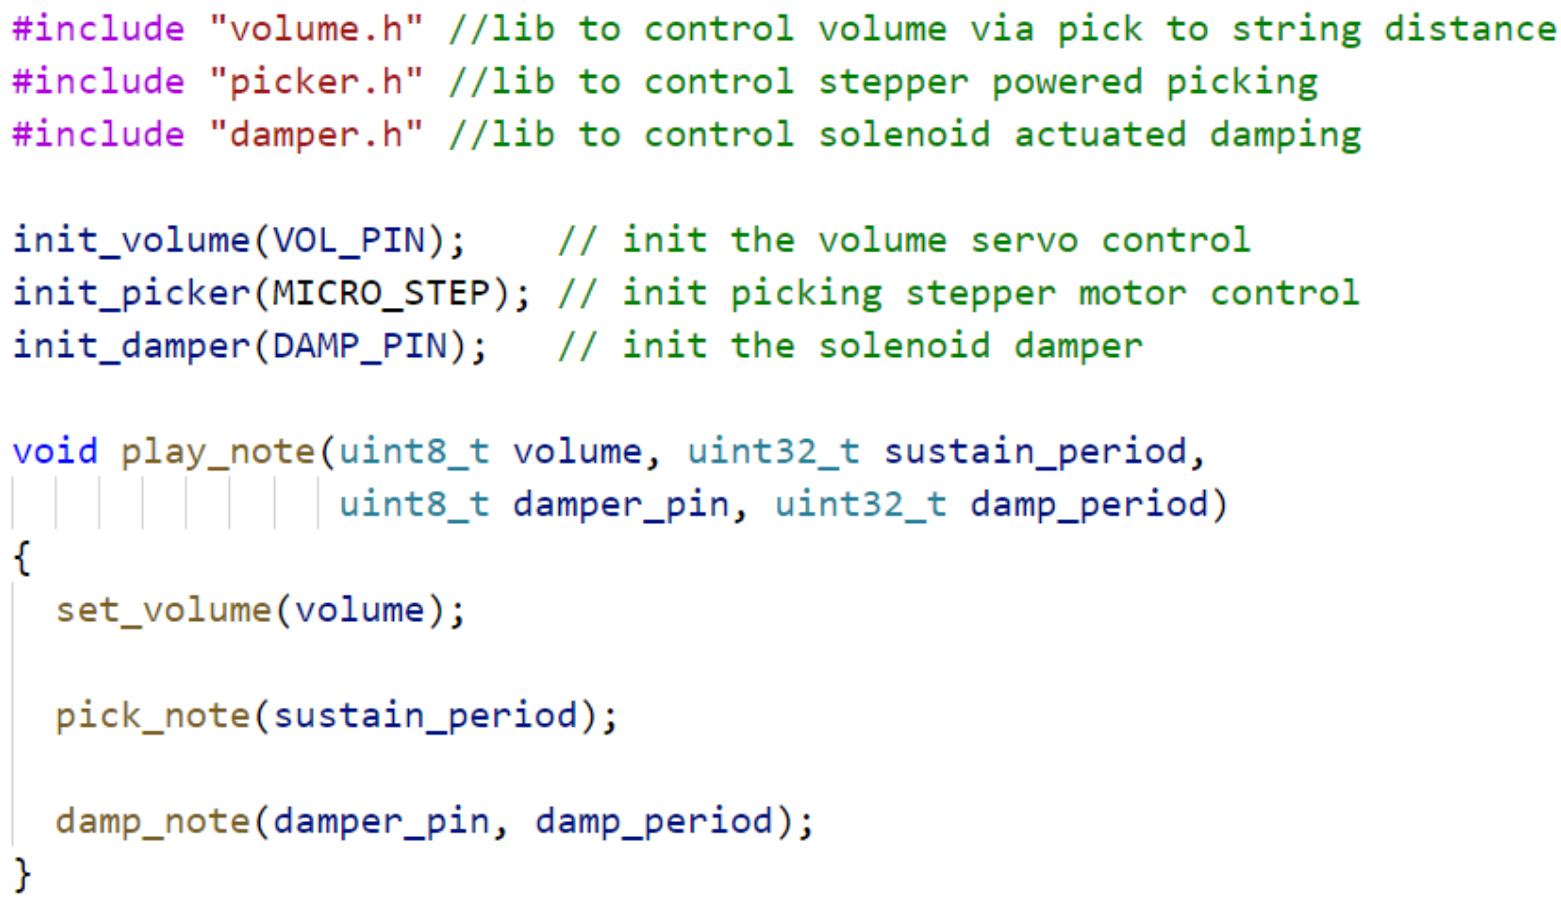
\includegraphics[width=0.7\textwidth]{code}
    \label{F:code}
    \caption{API Implementation}
  \end{center}
\end{figure}

\section{Proposed System Evaluation}

Due to COVID-19 restrictions, the implementation and evaluation of our designed system has been impractical, however the following sections will attempt to outline the evaluation that should be performed on our system.

\subsection{Picker Evaluation}

To be able to confirm the elimination of the audible backlash sound, a recording of audio from the magnetic pick-up, and audio from within the room should be taken while the picker is operating. This should then be compared to similar recordings taken from an existing "pick-wheel" picker such as the those found on MechBass \cite{McVay2015}. By comparing the ambient audio recorded within the room in a audio-visualiser such as Audacity, we can compare and identify if the clicking audio has been removed. Then by comparing the audio envelopes of the magnetic pick-up recordings we can identify if the improved designed has altered the pick profile. Ideally we will see that the audio envelopes between pickers remain constant, while the in person unwanted audio of the picker will be reduced.\\

Next, to evaluate the robustness of the clamping mechanism, the picker should be operated for an extended period of time, and then the start and end positions of the picks after this operation should be observed. This should be compared to the displacement produced by existing designs.

\subsection{Damper Evaluation}

To evaluate the performance of the damper, it will be important to compare it to the standard single point of contact dampers found in \cite{Carnegie2017}, as well as the original pinching design from \cite{kapur_history_nodate}.\\

A series of tests should be performed using these three damping types, and their pick-damp envelope profiles and in room audio should be recorded. By comparing the pick-damp envelope profile of the new design to that of the standard single contact damper, we will be able to identify if the new design is capable of eliminating noise due to string displacement.\\

Next, by comparing the in room audio of our design to that of the original pinch damper, we can identify if the spring design successfully mitigates the audible noise of the two dampers colliding.\\

Finally, but intentionally adding slight misalignments to our damper, and comparing it's pick-damp envelop to a properly aligned damper, we can observe if our design is more resilient and robust when compared to the original pinch damper.


\section{Conclusion}

To conclude, this project has managed to redesign existing picking and damping mechanisms to try and improve their performance and robustness. 

There has been a successful redesign of a "pick-wheel" based picking mechanism in which we have attempted to improve the acoustic qualities through the used of damping cushions, and improve it's reliability with updated pick slots and clamps. 

There has also been a successful redesign of the damping mechanism, integrating a pinching damper with a spring based contact. This strives to again improve the acoustic qualities of the damper, as well as provide damping without string displacement while mitigating misalignment. 

\newpage
\bibliographystyle{ieeetr}
\bibliography{references}

\end{document}